\documentclass{article}
\usepackage{tabularx}
\usepackage{amsmath}
\usepackage{here}
\usepackage{graphicx}
\usepackage[margin=2cm]{geometry}
\usepackage{cite}
\usepackage[final]{hyperref}
\usepackage{listings}
\hypersetup{
	colorlinks=true,
	linkcolor=blue,
	citecolor=blue,
	filecolor=magenta,
	urlcolor=blue         
}

\begin{document}

\title{Project\\An ant simulation}
\maketitle

\section{Introduction}
The project is an ant simulation. Ants must leave the anthill to find some resources. The only ability they have is to put pheromone on the floor.
\begin{figure}[H]
	\centering
	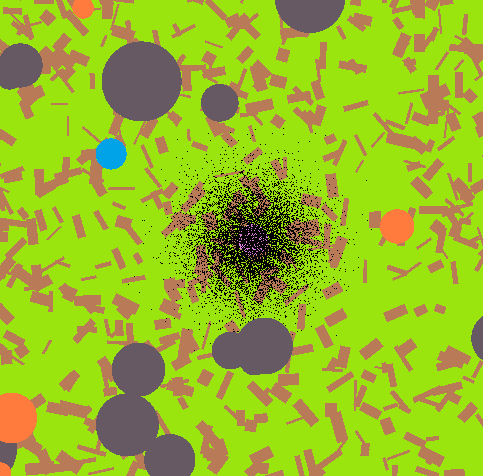
\includegraphics[scale=0.5]{figures/ant.png}
	\caption{The ant simulation}
\end{figure}

The initial code of the project can be find in this git repository:
\begin{lstlisting}
	https://github.com/robinfaurypro/GPGPU_ISIMA_2021-2022.git
\end{lstlisting}

For this simulation, we will use a real time application. The CUDA part will compute the image to show as fast as possible and OpenGL will print this image on the screen. Working with image is more complex than working with buffer. For the moment we use only buffer to keep simple. However, to print on the screen a buffer, we need first to convert it as a texture. A better option is to work directly with texture. GPU texture can be seen in the same way than buffer, but they come with a collection of tool (interpolation, repeat, ...).\\
For this project, we ask OpenGL to generate the texture to show and we use the interop feature to convert it into a surface. Surfaces can be send to the kernel in the same way than buffers. You can create a float4 on the kernel to fill the surface with your color.
\begin{lstlisting}
	__global__  void kernel_draw_map(cudaSurfaceObject_t surface) {
		int32_t x = blockIdx.x * blockDim.x + threadIdx.x;
		int32_t y = blockIdx.y * blockDim.y + threadIdx.y;
		float4 color = make_float4(0.6f, 0.9f, 0.05f, 1.0f);
		surf2Dwrite(color, surface, x * sizeof(float4), y);
	}
\end{lstlisting}

\section{Drawing the map}
The CUDA languages support the struct keyword. You can create a struct for the rock or the tree or the water and use thus structures in your kernel.
\begin{lstlisting}
	struct Tree {
		float u;
		float v;
		float radius;
	};
\end{lstlisting}
\begin{lstlisting}
	__global__ 
	void kernel_draw_map(cudaSurfaceObject_t surface, Tree* trees, int32_t nbTrees)
\end{lstlisting}
Generate a random map by using the std::uniform\_real\_distribution tool.

\end{document}